% Options for packages loaded elsewhere
\PassOptionsToPackage{unicode}{hyperref}
\PassOptionsToPackage{hyphens}{url}
\PassOptionsToPackage{dvipsnames,svgnames,x11names}{xcolor}
%
\documentclass[
  a4paper,
  stu,
  floatsintext,
  donotrepeattitle]{apa7}

\usepackage{amsmath,amssymb}
\usepackage{iftex}
\ifPDFTeX
  \usepackage[T1]{fontenc}
  \usepackage[utf8]{inputenc}
  \usepackage{textcomp} % provide euro and other symbols
\else % if luatex or xetex
  \usepackage{unicode-math}
  \defaultfontfeatures{Scale=MatchLowercase}
  \defaultfontfeatures[\rmfamily]{Ligatures=TeX,Scale=1}
\fi
\usepackage{lmodern}
\ifPDFTeX\else  
    % xetex/luatex font selection
\fi
% Use upquote if available, for straight quotes in verbatim environments
\IfFileExists{upquote.sty}{\usepackage{upquote}}{}
\IfFileExists{microtype.sty}{% use microtype if available
  \usepackage[]{microtype}
  \UseMicrotypeSet[protrusion]{basicmath} % disable protrusion for tt fonts
}{}
\makeatletter
\@ifundefined{KOMAClassName}{% if non-KOMA class
  \IfFileExists{parskip.sty}{%
    \usepackage{parskip}
  }{% else
    \setlength{\parindent}{0pt}
    \setlength{\parskip}{6pt plus 2pt minus 1pt}}
}{% if KOMA class
  \KOMAoptions{parskip=half}}
\makeatother
\usepackage{xcolor}
\setlength{\emergencystretch}{3em} % prevent overfull lines
\setcounter{secnumdepth}{-\maxdimen} % remove section numbering
% Make \paragraph and \subparagraph free-standing
\ifx\paragraph\undefined\else
  \let\oldparagraph\paragraph
  \renewcommand{\paragraph}[1]{\oldparagraph{#1}\mbox{}}
\fi
\ifx\subparagraph\undefined\else
  \let\oldsubparagraph\subparagraph
  \renewcommand{\subparagraph}[1]{\oldsubparagraph{#1}\mbox{}}
\fi


\providecommand{\tightlist}{%
  \setlength{\itemsep}{0pt}\setlength{\parskip}{0pt}}\usepackage{longtable,booktabs,array}
\usepackage{calc} % for calculating minipage widths
% Correct order of tables after \paragraph or \subparagraph
\usepackage{etoolbox}
\makeatletter
\patchcmd\longtable{\par}{\if@noskipsec\mbox{}\fi\par}{}{}
\makeatother
% Allow footnotes in longtable head/foot
\IfFileExists{footnotehyper.sty}{\usepackage{footnotehyper}}{\usepackage{footnote}}
\makesavenoteenv{longtable}
\usepackage{graphicx}
\makeatletter
\def\maxwidth{\ifdim\Gin@nat@width>\linewidth\linewidth\else\Gin@nat@width\fi}
\def\maxheight{\ifdim\Gin@nat@height>\textheight\textheight\else\Gin@nat@height\fi}
\makeatother
% Scale images if necessary, so that they will not overflow the page
% margins by default, and it is still possible to overwrite the defaults
% using explicit options in \includegraphics[width, height, ...]{}
\setkeys{Gin}{width=\maxwidth,height=\maxheight,keepaspectratio}
% Set default figure placement to htbp
\makeatletter
\def\fps@figure{htbp}
\makeatother

\usepackage{booktabs}
\usepackage{longtable}
\usepackage{array}
\usepackage{multirow}
\usepackage{wrapfig}
\usepackage{float}
\usepackage{colortbl}
\usepackage{pdflscape}
\usepackage{tabu}
\usepackage{threeparttable}
\usepackage{threeparttablex}
\usepackage[normalem]{ulem}
\usepackage{makecell}
\usepackage{xcolor}
\usepackage{tikz}
\usetikzlibrary{positioning}
\affiliation{{Utrecht University}}
\course{Methodology and Statistics for the Behavioral, Biomedical, and Social Sciences\\
Research Report}
\shorttitle{Confounding in Cross-Lagged Panel Models}
\duedate{22 Dec 2023}
\note{Student Number: 6100252\\
2499 words}
\professor{Supervisors: Ellen Hamaker, Jeroen Mulder}
\raggedbottom
\makeatletter
\@ifpackageloaded{tikz}{}{\usepackage{tikz}}
\makeatother
\makeatletter
\makeatother
\makeatletter
\@ifpackageloaded{caption}{}{\usepackage{caption}}
\AtBeginDocument{%
\ifdefined\contentsname
  \renewcommand*\contentsname{Table of contents}
\else
  \newcommand\contentsname{Table of contents}
\fi
\ifdefined\listfigurename
  \renewcommand*\listfigurename{List of Figures}
\else
  \newcommand\listfigurename{List of Figures}
\fi
\ifdefined\listtablename
  \renewcommand*\listtablename{List of Tables}
\else
  \newcommand\listtablename{List of Tables}
\fi
\ifdefined\figurename
  \renewcommand*\figurename{Figure}
\else
  \newcommand\figurename{Figure}
\fi
\ifdefined\tablename
  \renewcommand*\tablename{Table}
\else
  \newcommand\tablename{Table}
\fi
}
\@ifpackageloaded{float}{}{\usepackage{float}}
\floatstyle{ruled}
\@ifundefined{c@chapter}{\newfloat{codelisting}{h}{lop}}{\newfloat{codelisting}{h}{lop}[chapter]}
\floatname{codelisting}{Listing}
\newcommand*\listoflistings{\listof{codelisting}{List of Listings}}
\makeatother
\makeatletter
\@ifpackageloaded{caption}{}{\usepackage{caption}}
\@ifpackageloaded{subcaption}{}{\usepackage{subcaption}}
\makeatother
\makeatletter
\@ifpackageloaded{tcolorbox}{}{\usepackage[skins,breakable]{tcolorbox}}
\makeatother
\makeatletter
\@ifundefined{shadecolor}{\definecolor{shadecolor}{rgb}{.97, .97, .97}}
\makeatother
\makeatletter
\makeatother
\makeatletter
\makeatother
\ifLuaTeX
  \usepackage{selnolig}  % disable illegal ligatures
\fi
\usepackage[style=apa]{biblatex}
\addbibresource{Masterscriptie.bib}
\IfFileExists{bookmark.sty}{\usepackage{bookmark}}{\usepackage{hyperref}}
\IfFileExists{xurl.sty}{\usepackage{xurl}}{} % add URL line breaks if available
\urlstyle{same} % disable monospaced font for URLs
\hypersetup{
  pdftitle={One Step Toward Causality: Unobserved Time-Invariant Confounding in Cross-Lagged Panel Models},
  pdfauthor={Pepijn A. Vink},
  pdfkeywords={RI-CLPM, DPM, causality, longitudinal, simulation, confounding},
  colorlinks=true,
  linkcolor={blue},
  filecolor={Maroon},
  citecolor={Blue},
  urlcolor={Blue},
  pdfcreator={LaTeX via pandoc}}

\title{One Step Toward Causality: Unobserved Time-Invariant Confounding
in Cross-Lagged Panel Models}
\author{Pepijn A. Vink}
\date{}

\begin{document}
\maketitle
\ifdefined\Shaded\renewenvironment{Shaded}{\begin{tcolorbox}[borderline west={3pt}{0pt}{shadecolor}, boxrule=0pt, breakable, sharp corners, frame hidden, enhanced, interior hidden]}{\end{tcolorbox}}\fi

\newcommand{\indep}{\perp \!\!\! \perp}

\hypertarget{introduction}{%
\section{Introduction}\label{introduction}}

Cross-lagged panel designs, which are based on measuring the same
individuals on the same variables for two or more occasions, are
commonly used in psychological research to investigate relationships
between multiple constructs over time. Several longitudinal SEM models
have been developed for analyzing such data, of which the random
intercept cross-lagged panel model
\autocites[RI-CLPM,][]{hamaker2015,mulder2021} is one of the most
popular. The RI-CLPM, shown in Figure \ref{fig:riclpm}, decomposes
observed variables into stable between-person differences and temporal
within-person components, and the dynamics are modeled using these
within-person components. Usually, the effects of the variables on each
other at later timepoints, the cross-lagged effects, are most of
interest. These are often interpreted as causal effects, albeit
implicitly. However, a causal interpretation presumes that both
time-varying and time-invariant confounders are adequately controlled
for, an assumption commonly referred to as absence of unobserved
confounding.

\textcite{usami2019} show that when certain assumptions are met, the
random intercept in the RI-CLPM controls for unobserved heterogeneity
resulting from confounding. This requires, in particular, that the
confounders are time-invariant, and that the effects of the confounders
on the variables of interest are stable over time. However, it has not
yet been studied how the RI-CLPM performs when the effects of unobserved
time-invariant confounders are of a time-varying nature.
\textcite{murayama2022} show that the Dynamic Panel Model (DPM), shown
in Figure \ref{fig:dpm}, may be an alternative in this case. This model
is similar to the RI-CLPM due to the inclusion of lagged effects as well
as a latent component, but the dynamics are now situated between the
observed variables, rather than between within-person components. While
some prefer this model because it is less restrictive and it is claimed
to better control for unobserved confounding \autocite{allison2017},
others would regard the absence of an explicit within-between
decomposition as a downside \autocite[e.g.][]{hoffman2024}. Furthermore,
it is unknown how either of these models perform when the underlying
causal process is more complex, for example when multiple confounders
with time-varying effects are involved.

\begin{figure}

\caption{\label{fig-models}Structural Equation Model Representations of
Two Popular Models in Panel Research}\begin{minipage}[t]{\linewidth}
\subcaption{\label{fig:riclpm}Random Intercept Cross-Lagged Panel Model
(RI-CLPM)\textsuperscript{a}}

{\centering 

\raisebox{-\height}{

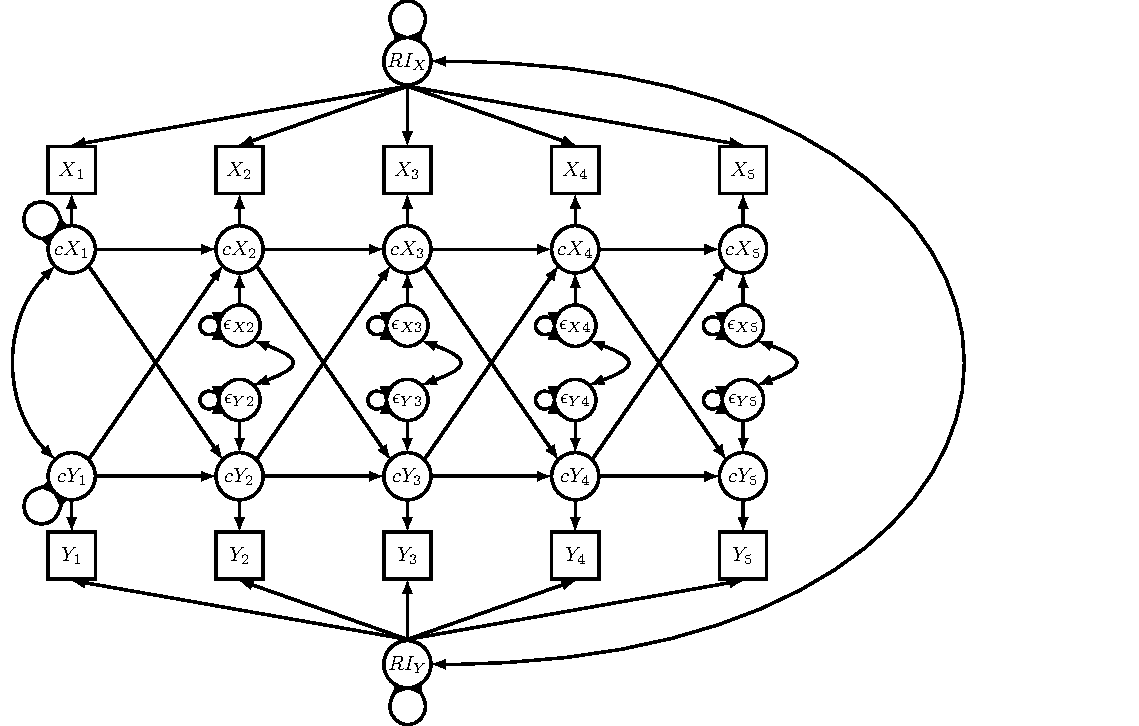
\includegraphics[width=0.9\textwidth]{riclpm_cropped.pdf}

}

}

\end{minipage}%
\newline
\begin{minipage}[t]{\linewidth}
\subcaption{\label{fig:dpm}Dynamic Panel Model (DPM)}

{\centering 

\raisebox{-\height}{

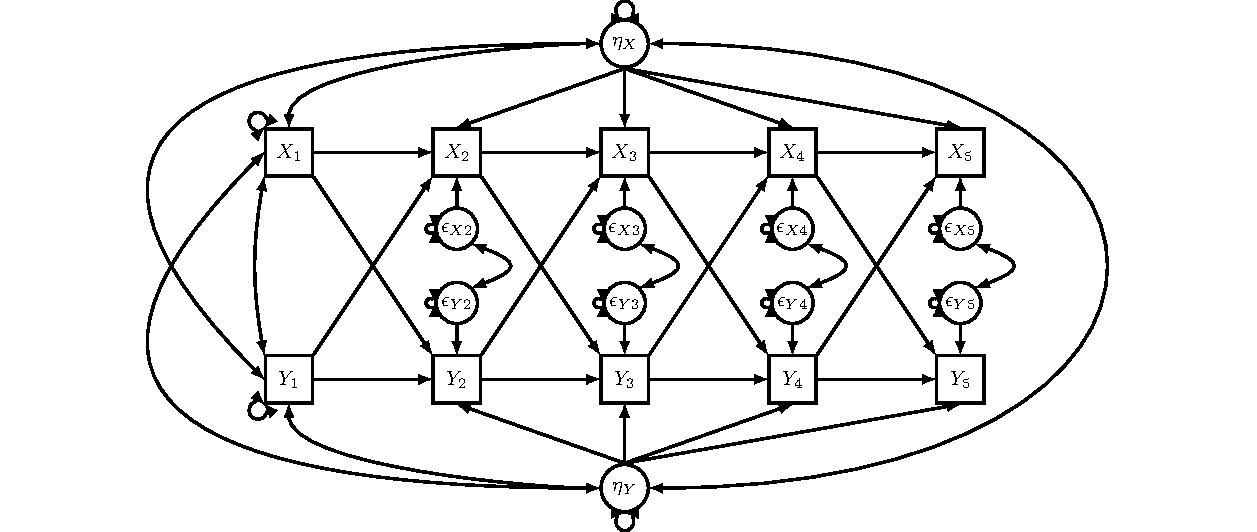
\includegraphics[width=0.9\textwidth]{dpm_cropped.pdf}

}

}

\end{minipage}%
\newline
\begin{minipage}[t]{\linewidth}

{\centering 

\begin{flushleft}
\textit{Note}. Boxes Indicate Observed Variables
and Circles Indicate Latent Variables.

$^a$ Observed Scores are Decomposed into a Stable Person-Specific
Component ($RI_X$ and $RI_Y$), and Within-Person Components ($cX$ and
$cY$).
\end{flushleft}

}

\end{minipage}%

\end{figure}

Therefore, the effect of time-invariant confounders on both the RI-CLPM
and the DPM should be explored further. This research report will
evaluate the extent to which unobserved time-invariant confounders
affect the estimates of the RI-CLPM and DPM. Specifically, we will
assess whether these estimates give a good indication of underlying
causal effects when multiple unobserved time-invariant confounders are
involved.

This report is structured as follows. We start with a conceptual
comparison between the RI-CLPM and the DPM. Then, a hypothetical causal
model that includes multiple time-invariant confounders is introduced.
This model is used as the data generating mechanism for a simulation
study that evaluates the performance of the RI-CLPM and the DPM under
the data generating mechanism. We end with a discussion of results and
implications.

\hypertarget{a-comparison-of-the-ri-clpm-and-the-dpm}{%
\section{A Comparison of the RI-CLPM and the
DPM}\label{a-comparison-of-the-ri-clpm-and-the-dpm}}

The RI-CLPM is commonly used with the goal to investigate causal
relationships between variables while accounting for stable
between-person differences \autocite{hamaker2015}. It decomposes the
observed scores of an individual into a stable person-specific deviation
from the grand mean, and a temporal deviation from this stable component
by including a random intercept factor. These temporal deviations make
up the `within' part of the RI-CLPM where the dynamics are modeled. As
Figure \ref{fig:riclpm} shows, this factor only has direct effects on
the observed variables, and no effect on the observed scores of the
other variable. The random intercept of \(X\) is only related to the
observed scores of \(Y\) through a covariance between the random
intercepts, and vice versa.

Likewise, the DPM is also used to estimate causal relationships between
variables over time. However, the DPM does this while aiming to control
for unmeasured time-invariant confounders \autocite{allison2017}. It
does not explicitly separate within person dynamics from stable between
person differences, and lagged effects are included on the observed
scores. The latent factors in the DPM are sometimes called `accumulating
factors' \autocite{usami2019}, as their effects on the observed
variables are both direct, as well as indirect through lagged
relationships between the observed variables themselves, a property that
becomes clear from Figure \ref{fig:dpm}. To account for the fact that
measurements are usually sampled at a random moment in time in an
ongoing process, the observations at the first timepoints are often
allowed to covary freely with each other and the accumulating factors
\autocite{hamaker2005}, which is not necessary in the RI-CLPM.

\textcite{hamaker2005} shows that under certain circumstances, the
RI-CLPM and the DPM are statistically equivalent and yield equivalent
estimates of the lagged parameters. This is the case when lagged
parameters are invariant over time, and the factor loadings in the DPM
at the first timepoint are constrained to reflect this, rather than
specified as free covariances. This also implies that when these
conditions hold in a data generating mechanism, the RI-CLPM and the DPM
should both yield unbiased estimates. However, it is yet unknown how the
estimates behave when the underlying mechanism is more complex.

\hypertarget{methods}{%
\section{Methods}\label{methods}}

Although there is information on the behavior of the RI-CLPM and the DPM
in simple cases of unobserved confounding, as is discussed in the
previous section, it is yet unknown how the estimates behave when the
underlying mechanism is more complex. Therefore, we present a simulation
study to assess the performance of the RI-CLPM and the DPM under
different patterns of unobserved confounding. We first introduce a
causal model that includes multiple confounders. This serves as a
general data generating mechanism for the simulations. Three different
scenarios are considered, which differ with respect to the stability of
the effects of the confounders.

\hypertarget{the-causal-model}{%
\subsection{The Causal Model}\label{the-causal-model}}

To represent the causal model that we simulated, we use the causal
directed acyclic graph (DAG) in Figure~\ref{fig-scm}. It shows a dynamic
process for \(t=1,...,5\) between time-varying variables \(X\) and \(Y\)
and includes two time-invariant baseline confounders, \(C_1\) and
\(C_2\), that each have an effect on all future observations of \(X\)
and \(Y\). The structure of the DAG is most similar to the dynamic panel
model, as observed values are determined by observed values at previous
timepoints, but it may also represent confounding on the within-person
dynamics in the RI-CLPM. However, it should be noted that this DAG is
not equivalent to either model, as each confounder has effects on both
\(X\) and \(Y\), whereas the latent factors in the RI-CLPM and DPM are
variable-specific.

\begin{figure}

\caption{\label{fig-scm}Directed Acyclic Graph for Cross-Lagged
Relationships Between \(X\) and \(Y\) at Multiple Timepoints.
Confounders \(C_1\) and \(C_2\) Have Effects on Both \(X\) and \(Y\) at
Each Timepoint. Dashed Lines Indicate the Process Before the Observed
Timepoints}

{\centering 

\usetikzlibrary{positioning}
\usetikzlibrary{arrows}
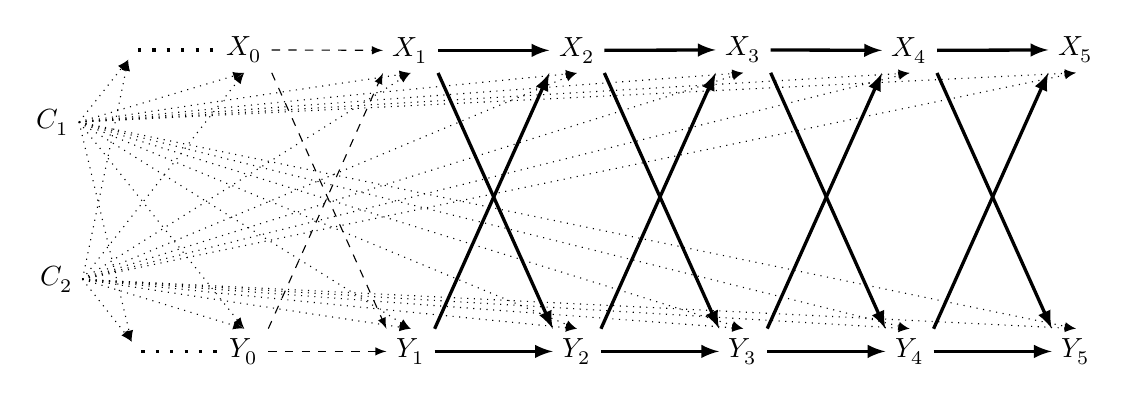
\begin{tikzpicture}[auto,node distance=.5cm, scale=0.5,
paths/.style={->, very thick, -latex},
dot/.style={dotted, ->, -latex},
double/.style={very thick, latex-latex},
dashpath/.style={dashed, ->, -latex}
]
%create nodes
\node (y1) at (0,0) {};
\node[right=1cm of y1] (yt) {$Y_0$};
\node[right=1.5cm of yt] (y2) {$Y_{1}$};
\node[right=1.5cm of y2] (y3){$Y_{2}$};
\node[right=1.5cm of y3] (y4){$Y_{3}$};
\node[right=1.5cm of y4] (y5){$Y_{4}$};
\node[right=1.5cm of y5] (y6){$Y_{5}$};

\node[above=1.5cm of yt] (ut){};
\node[above=1.5cm of y2] (u2){};
\node[above=1.5cm of y3] (u3){};
\node[above=1.5cm of y4] (u4){};
\node[above=1.5cm of y5] (u5){};
\node[above=1.5cm of y6] (u6){};

\node[above=1.5cm of ut] (xt){$X_0$};
\node[left=1cm of xt] (x1){};
\node[above=1.5cm of u2] (x2){$X_{1}$};
\node[above=1.5cm of u3] (x3){$X_{2}$};
\node[above=1.5cm of u4] (x4){$X_{3}$};
\node[above=1.5cm of u5] (x5){$X_{4}$};
\node[above=1.5cm of u6] (x6){$X_{5}$};

\node[below left=0.5cm and 0.5cm of x1] (c1){$C_{1}$};
\node[above left=0.5cm and 0.5cm of y1] (c2){$C_{2}$};

%draw paths
\draw[dashpath] (xt.south east) -- (y2.north west);
\draw[dashpath] (yt.north east) -- (x2.south west);

\draw[paths] (x2.south east) -- (y3.north west);
\draw[paths] (x3.south east) -- (y4.north west);
\draw[paths] (x4.south east) -- (y5.north west);
\draw[paths] (x5.south east) -- (y6.north west);
\draw[paths] (y2.north east) -- (x3.south west);
\draw[paths] (y3.north east) -- (x4.south west);
\draw[paths] (y4.north east) -- (x5.south west);
\draw[paths] (y5.north east) -- (x6.south west);

\draw[loosely dotted, very thick] (x1.east) -- (xt.west);
\draw[dashpath] (xt.east) -- (x2.west);
\draw[paths] (x2.east) -- (x3.west);
\draw[paths] (x3.east) -- (x4.west);
\draw[paths] (x4.east) -- (x5.west);
\draw[paths] (x5.east) -- (x6.west);
\draw[loosely dotted, very thick] (y1.east) -- (yt.west);
\draw[dashpath] (yt.east) -- (y2.west);
\draw[paths] (y2.east) -- (y3.west);
\draw[paths] (y3.east) -- (y4.west);
\draw[paths] (y4.east) -- (y5.west);
\draw[paths] (y5.east) -- (y6.west);

\draw[dot] (c1.east) -- (x1.south);
\draw[dot] (c1.east) -- (xt.south);
\draw[dot] (c1.east) -- (x2.south);
\draw[dot] (c1.east) -- (x3.south);
\draw[dot] (c1.east) -- (x4.south);
\draw[dot] (c1.east) -- (x5.south);
\draw[dot] (c1.east) -- (x6.south);

\draw[dot] (c1.east) -- (y1.north);
\draw[dot] (c1.east) -- (yt.north);
\draw[dot] (c1.east) -- (y2.north);
\draw[dot] (c1.east) -- (y3.north);
\draw[dot] (c1.east) -- (y4.north);
\draw[dot] (c1.east) -- (y5.north);
\draw[dot] (c1.east) -- (y6.north);

\draw[dot] (c2.east) -- (x1.south);
\draw[dot] (c2.east) -- (xt.south);
\draw[dot] (c2.east) -- (x2.south);
\draw[dot] (c2.east) -- (x3.south);
\draw[dot] (c2.east) -- (x4.south);
\draw[dot] (c2.east) -- (x5.south);
\draw[dot] (c2.east) -- (x6.south);

\draw[dot] (c2.east) -- (y1.north);
\draw[dot] (c2.east) -- (yt.north);
\draw[dot] (c2.east) -- (y2.north);
\draw[dot] (c2.east) -- (y3.north);
\draw[dot] (c2.east) -- (y4.north);
\draw[dot] (c2.east) -- (y5.north);
\draw[dot] (c2.east) -- (y6.north);

\end{tikzpicture}

}

\end{figure}

When the underlying dynamic process has stabilized around an
equilibrium, and when lagged effects as well as the effects of the
confounders are time-invariant, in both the RI-CLPM and the DPM the
latent factors will be a linear combination of the confounders
\autocite{usami2019}. Therefore, when these conditions hold, we expect
both models to yield unbiased estimates of the lagged effects, even when
the confounders are unobserved. However, when the effects of the
confounders are not time-stable, the models may not be able to fully
account for the effects of confounders, thus resulting in biased
effects.

This causal model was simulated to assess the performance of the RI-CLPM
and the DPM under different scenarios of confounding. These scenarios
were all simulated as special cases of the data generating mechanism in
Figure~\ref{fig-scm} and are represented by the following equations:

For person \(i\) at timepoint \(t\), \[
x_{it} = \phi_{xx}x_{i,t-1} + \phi_{xy}y_{i,t-1} + \gamma_{1t}C_{1i} + \gamma_{2t}C_{2i} + \epsilon_{xit},
\] \[
y_{it} = \phi_{yy}y_{i,t-1} + \phi_{yx}x_{i,t-1} + \delta_{1t}C_{1i} + \delta_{2t}C_{2i} + \epsilon_{yit}.
\]

Furthermore, at the first simulated timepoint, \[
x_{i} = \gamma_{1}C_{1i} + \gamma_{2}C_{2i} + \epsilon_{xi},
\] \[
y_{i} = \delta_{1}C_{1i} + \delta_{2}C_{2i} + \epsilon_{yi}.
\]

In addition, \[
\epsilon_{xt} \sim \mathcal{N}(0, \psi_x),
\] \[
\epsilon_{yt} \sim \mathcal{N}(0, \psi_y),
\] \[
C_{1} \sim \mathcal{N}(0, \psi_{C_1}),
\] \[
C_{2} \sim \mathcal{N}(0, \psi_{C_2}).
\]

From these equations follows that lagged effects and (residual)
variances are time-invariant, whereas effects of the confounders may be
time-varying, as indicated by the absence or presence of a time index
\(t\) for these parameters. In our simulation, for all scenarios, lagged
effects were set to \(\phi_{xx} =\) 0.2, \(\phi_{yy} =\) 0.3,
\(\phi_{xy} =\) 0.15, \(\phi_{yx} =\) 0.1 \autocite[based
on][]{mulder2023}, and (residual) variances were all set to 1.

Three scenarios were simulated. For all scenarios, at the start,
\(\gamma_{1} =\) 0.3, \(\gamma_{2} =\) 0.8, \(\delta_{1} =\) 0.5, and
\(\delta_{2} =\) 0.2. For scenario 1, the effects of the confounders
remain stable. For scenario 2, at \(t=3\), the effects of \(C_1\) on
\(x\) and \(y\) decrease, and remain stable afterwards (\(\gamma_{1} =\)
0.1 and \(\delta_{1} =\) 0.2). For scenario 3, at \(t=3\) all effects of
confounders change and afterwards remain stable. For \(C_1\) its effect
on \(x\) increases and its effect on \(y\) decreases (\(\gamma_{1} =\)
0.6 and \(\delta_{1} =\) 0.2), and vice versa for \(C_2\)
(\(\gamma_{2} =\) 0.3 and \(\delta_{2} =\) 0.5).

For each scenario, 1000 datasets were simulated with N=500. To allow for
convergence to an equilibrium, we simulated 50 timepoints, of which 45
were used as burn-in. The remaining 5 timepoints, \(t=1,...,5\), were
analyzed.

\hypertarget{analysis}{%
\subsection{Analysis}\label{analysis}}

To assess the performance of the RI-CLPM and the DPM when confounders
are unobserved, all simulated datasets were analyzed using the RI-CLPM
and the DPM, as well as versions of these models with free loadings for
the latent factors, because freeing the factor loadings may, in part,
capture the time-varying effects of the unobserved confounders. Models
that did not converge or did not result in positive definite covariance
matrices were excluded. All simulations and analyses were performed
using R version 4.3.2 \autocite{R}. Models were fit using the lavaan
package version 0.6-16 \autocite{lavaan}.

\hypertarget{results}{%
\section{Results}\label{results}}

The discussion of results focuses on the \(x_4 \rightarrow y_5\) effect
(\(\phi_{xy} = 0.1\)). For all models, for each scenario, the bias,
Monte-Carlo error, root mean squared error (RMSE), and coverage were
computed, based on recommendations by \textcite{morris2019}. The bias
was computed as the difference between the mean of the empirical
sampling distribution, that is, the distribution of our estimates, and
the true effect. The Monte-Carlo error was computed as the standard
error of this estimate, and the RMSE was computed as the root of the
mean squared deviation from the true value. Setting \(\alpha = 0.5\),
the coverage is the proportion of times that the 95\% confidence
interval contains the true value. The coverage is typically seen as
acceptable when it is close to 95\%.

Upon initial inspection of the models, we found that for scenario 3, a
high number of models resulted in a non positive-definite matrix of the
latent variables. Specifically, the random intercepts or accumulating
factors had a correlation higher than 1 in all of the RI-CLPM models and
in most of the DPM models (91.9\% and 55.8\% for the DPM without and
with free loadings, respectively). Therefore, for subsequent results,
the models were rerun, with correlations between random intercepts or
accumulating factors set to 1. It should be kept in mind, however, that
this constitutes an exploratory approach as it was not based on theory.
Therefore, results may not generalize well to other situations.

Table~\ref{tbl-measures} shows the relative bias, RMSE, and coverage for
the \(x_4 \rightarrow y_5\) effect for each model, in each scenario, and
Figure~\ref{fig-biases} visualizes the biases, with their corresponding
Monte-Carlo errors. Table~\ref{tbl-measures} and Figure~\ref{fig-biases}
show that under scenario 1, as expected, both the RI-CLPM and the DPM
yield unbiased estimates. Surprisingly, freeing the factor loadings
results in bias. Specifically, they yield a negative bias, indicating
that the effect is underestimated. Furthermore, the DPM has a lower RMSE
than the RI-CLPM, indicating that under this scenario, the DPM shows
less average absolute deviation from the true effect and thus may be a
better choice. All coverages are relatively acceptable.

Under scenario 2, where the effects of \(C_1\) are time-varying, both
the RI-CLPM and the DPM yield biased estimates. Specifically, the
RI-CLPM shows a relatively extreme underestimation of the true effect,
and the DPM yields a small overestimation. Furthermore, freeing the
loadings does not capture the time-varying effects of the confounders,
as indicated by the extreme relative biases. The DPM has the lowest RMSE
of all models. The RI-CLPM shows very low coverage, and the RI-CLPM with
free loadings has coverage that may be too high.

Under scenario 3, where both confounders have time-varying effects, all
models show large bias. In this situation, the RI-CLPM and DPM with free
factor loadings have lower bias than their counterparts with fixed
loadings. Furthermore, RI-CLPM and the DPM have very low coverages, and
the versions with free factor loadings have coverages that may be too
high. The DPM yields the lowest RMSE.

\begin{figure}

\caption{\label{fig-biases}Biases for the Effect of \(x_4\) on \(y_5\)}

{\centering 

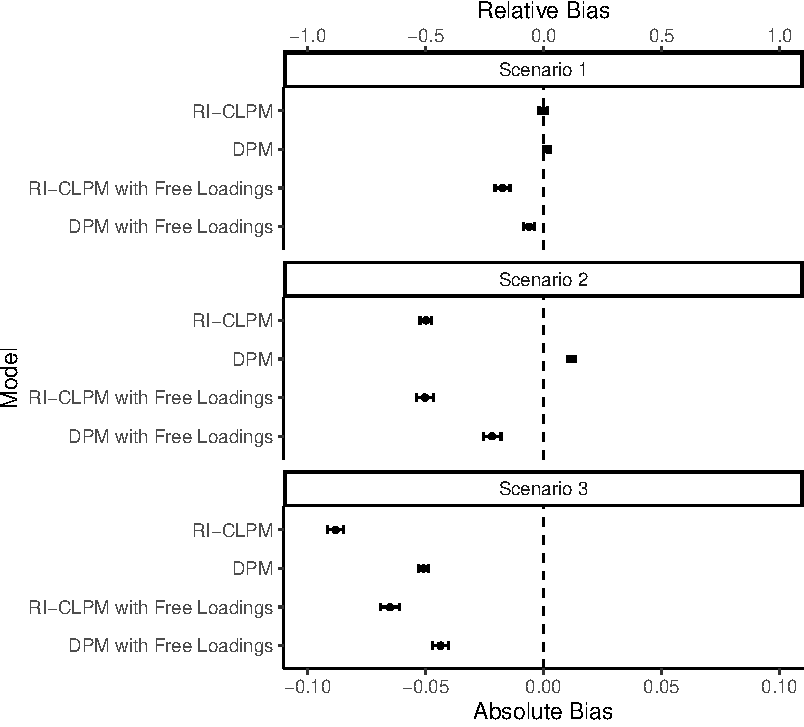
\includegraphics{research-report_files/figure-pdf/plot-bias-1.pdf}

\begin{flushleft}
\emph{Note.} The true effect is equal to \(\phi_{yx} = 0.1\). The Dots
indicate the (relative) bias of each model's estimates. The error bars
indicate the Monte-Carlo error.

\end{flushleft}

}

\end{figure}

\renewcommand{\arraystretch}{0.7}

\hypertarget{tbl-measures}{}
\begin{table}
\caption{\label{tbl-measures}Relative Bias, RMSE, and Covarage for Each Scenario on the Effect of
\(x_4\) on \(y_5\). The True Effect is 0.1 }\tabularnewline

\centering
\begin{tabular}{llccc}
\toprule
Scenario & Model & Relative Bias (\%) & RMSE\textsuperscript{1} & Coverage (\%)\textsuperscript{2}\\
\midrule
 & RI-CLPM & -0.11 & 0.06 & 94.40\\

 & DPM & 1.52 & 0.04 & 95.69\\

 & RI-CLPM (free loadings) & -17.39 & 0.10 & 95.81\\

\multirow{-4}{*}{\raggedright\arraybackslash 1} & DPM (free loadings) & -6.06 & 0.07 & 94.73\\
\cmidrule{1-5}
 & RI-CLPM & -49.81 & 0.08 & 88.94\\

 & DPM & 11.83 & 0.04 & 94.52\\

 & RI-CLPM (free loadings) & -50.27 & 0.11 & 97.78\\

\multirow{-4}{*}{\raggedright\arraybackslash 2} & DPM (free loadings) & -21.80 & 0.09 & 95.42\\
\cmidrule{1-5}
 & RI-CLPM & -88.09 & 0.11 & 71.70\\

 & DPM & -50.86 & 0.07 & 79.10\\

 & RI-CLPM (free loadings) & -65.04 & 0.12 & 98.00\\

\multirow{-4}{*}{\raggedright\arraybackslash 3} & DPM (free loadings) & -43.64 & 0.10 & 96.65\\
\bottomrule
\multicolumn{5}{l}{\rule{0pt}{1em}\textsuperscript{1} Root Mean Square Error.}\\
\multicolumn{5}{l}{\rule{0pt}{1em}\textsuperscript{2} Inclusion frequency of the true effect for the 95\% confidence interval.}\\
\end{tabular}
\end{table}

\hypertarget{discussion}{%
\section{Discussion}\label{discussion}}

Previous research has suggested that when lagged effects and the effects
of unobserved time-invariant confounders are stable over time, both the
RI-CLPM and the DPM yield unbiased estimates of the true cross-lagged
effect, even when the confounders are unobserved
\autocite[e.g.][]{usami2019}. This characteristic of both models was
replicated by the discussed simulations in scenario 1. However, the
extent to which this is a reasonable causal model is debatable. For many
phenomena, it may be more realistic to assume effects of confounders to
vary over time.

Therefore, we also considered situations where effects of one or two
confounders changed over time. In our simulations, the RI-CLPM and the
DPM respectively underestimated and overestimated the cross-lagged
effects when this was the case. Furthermore, freeing the factor loadings
in both models did not fully capture the time-varying nature as negative
bias was observed in these models as well. However, because only few
scenarios were considered, we cannot yet conclude that these models
generally underestimate cross-lagged effects when confounders are
unobserved; other data generating mechanisms may show different
patterns. Furthermore, although bias in the estimates was present in
these scenarios, conclusions on the direction of the effect generally
did not change, as the estimated effects were still positive.

The analyses performed in our simulation were used on simulated data
with unobserved confounders. When confounders are measured, however, it
may be more appropriate to model them explicitly. This can be done by
including them in the model as covariates \autocite{mulder2021}, but
methods specifically designed for causal inference may be more fitting
\autocite{schafer2008a,leite2019}, especially when many confounders are
involved or when effects are nonlinear. In reality, however, only a
subset of confounders are likely observed, while others remain
unobserved. In such situations, it could be advantageous to use a
combination of methods, such as using the RI-CLPM or DPM to correct for
some unobserved confounders, and use propensity score based causal
inference methods to correct for observed confounders. However, the
extent to which this is possible and sensible is yet to be explored.

We should therefore investigate whether the toolbox of social science
researchers can be expanded by integrating causal inference methods with
cross-lagged panel models, which will be covered by the thesis. The
presented results highlight the necessity of such research and emphasize
the importance of acting with caution when attempting to assess cause
and effect.

\newpage{}

\hypertarget{references}{%
\section*{References}\label{references}}
\addcontentsline{toc}{section}{References}

\printbibliography[heading=none]




\end{document}
